\documentclass[../../Rapport RayTracer]{subfiles}

\begin{document}

La méthode retenu pour effectuer le parsing d'un fichier POV est celle de l'automate à états finis. C'est donc pour cela que l'on a crée la classe Automat. Le principe est simple, on associe à chaque figure une classe d'état. Une classe EtatSphere, une classe EtatTriangle, etc. Chaque classe d'état s'occupe de parser son objet associé. La classe Automat s'occupe juste d'appeler au bon moment les états, c'est à dire quand le jeton de son StreamTokenizer rencontre un mot connu, soit sphère, plane, box... Les différents états possibles de l'automate sont définis dans l'énumération State. 
Voici le diagramme d'états des figures:

\begin{figure}[h!]
	\adjustbox{center}{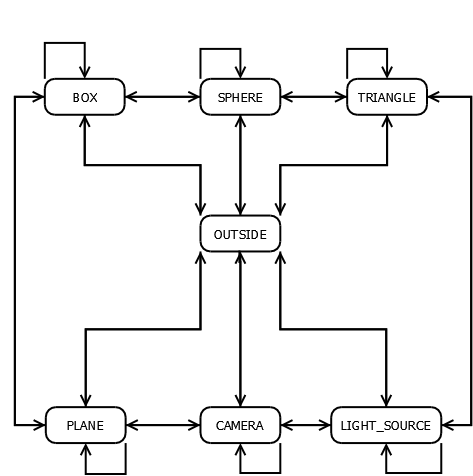
\includegraphics[width=0.75\textwidth]{diagrammes/Diagramme_etat.png}}
	
	\caption{Diagramme d'étas des figures}
	\label{diagrammeEtatFigure}
\end{figure}
\FloatBarrier


Concrètement, dans la classe Automat, on traverse le fichier jusqu'à ce qu'on rencontre une figure connu. A ce moment là, on fixe l'état sur cette figure et on appelle la classe d'état correspondante. Dès lors que la parsing de la figure est fini, on regarde le prochain mot et on fixe l'état correspondant. Tout ces traitements dont effectués dans une boucle qui a pour condition de d'arrêt la fin du fichier. Ensuite on switch sur l'état courant et on définit autant de case qu'il y a d'états. On a aussi définit un état vide, l'état OUTSIDE qui correspond à aucun élément de syntaxe. Dès lors que l'on se trouve dans un état OUTSIDE, on avance juste notre jeton dans le fichier pour tomber sur la prochaine figure, s'il y en a une.
\begin{adjustbox}{max width=\textwidth}
 \lstinputlisting[language=Java]{../../code/automat.java}
\end{adjustbox} 
De plus nous avons implémenté des sous états qui se trouvent dans chaque classe. Ils sont contenus dans des énumérations présentes dans chaque classe d'états. Ces états correspondent en fait à des éléments de syntaxe que l'on trouve dans un bloc de figure. C'est à dire qu'on a un état pour l'accolade fermante, ouvrante, le chevron ouvrant , le chevron fermant etc.
Le principe est le même que pour les états de figures. Même s'ils se ressemblent fortement, nous avons besoin d'une énumération par classe car la syntaxe n'est pas toujours la même pour chaque figure.
\\

Par ailleurs, pour des raisons de factorisation, nous avons ajouté un état ATTRIBUTE. En effet, quelque soit la figure sur laquelle on se trouve, si elle possède un bloc finish (lumière) ou un bloc pigment (couleurs), la syntaxe sera la même peu importe la figure. C'est donc pour cela que l'on a crée un classe EtatUtil qui s'occupe de parser ces autres blocs de code. En fait chaque classe d'état parse les coordonées de sa figure et appelle la classe mère EtatUtil en lui donnant le contexte courant pour parser ses attributs s'il y en a. Toutes les classes d'état héritent donc de la classe mère EtatUtil

\end{document}
